\chapter{More Complex Formulas}
The formulas in the previous section are common formulas, however they are fairly simple and only cover a small subset of the infinite amount of possible formulas that can be formed by temporal logics. The benefit of using temporal logics is that a wide variety of behaviours can be expressed, including propositions about the robot \textit{and} about the workspace. Up to now, we have not looked at any formulas that include atomic propositions about potential tasks. We will show through examples that the same ideas presented in the previous chapter still hold true for these complex tasks, and show the speed up we get by using the greedy algorithm compared to the accepted algorithm. 

\section{Example 1}
We look at the example from \cite{guo15} which says "eventually pick up the red ball. Once it is done, move to one basket and drop it. At last come back to room one and stay there". This task can be written as the LTL formula $\varphi = \diamond (\text{pickrball} \wedge \diamond \text{droprball}) \wedge \diamond \smallsquare r1$. The B\"uchi automaton corresponding to this formula as translated by \ref{fig:ex1SimplifiedBuchi}, with all edges that have \&\& in the label removed. For this example we will be using Workspace 2 shown in figure \ref{fig:workspace2}.

We note here pickrball and droprball are potential tasks i.e.\ they belong in $AP_p$. They are incoded in the action model in the P\_MAS\_TG framework. pickrball can only be done if rball is true, and this is only true in the region corresponding to (9,15).  droprball can only be done if basket1 is true, and this is only true in the region corresponding to (7,14) (see figure \ref{fig:workspace2}). We give both of these actions an arbitrary cost of 10. The way P\_MAS\_TG treats actions gives increases the size of the product automaton by three fold. This is because when a predicate is incoded as an action, each state has corresponding states for doing that action in this state. So instead of having a product automaton of size $|\text{FTS}| \times |\text{B\"uchi}| $ we have a size $|\text{FTS}| \times |\text{B\"uchi}| \times |\text{possible actions}|$. The possible actions in this case are \{ "none", "pickrball", "droprball" \}. We said that pickrball was only possible when rball is true and droprball is only possible when basket1 is true. This statement is still valid, the resulting contradictory nodes simply have no edges leading to them so they cannot be reached. 

%\begin{figure*}[!htb]
%\centering
%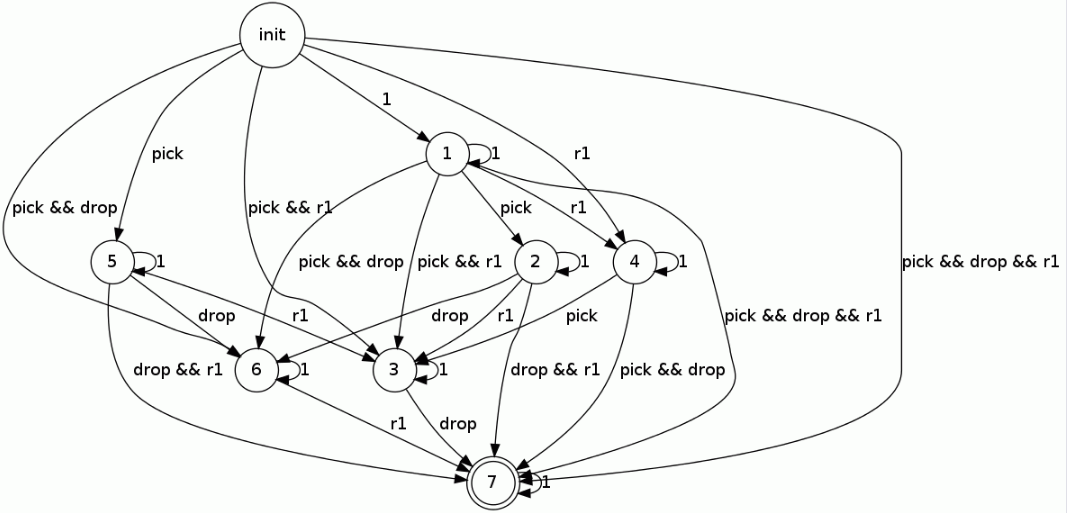
\includegraphics[scale=0.3]{buchiEx1_1}
%\caption{B\"uchi Automaton Corresponding to $\varphi = \diamond (\text{pickrball} \wedge \diamond \text{droprball}) \wedge \diamond %\smallsquare r1$}
%\label{fig:buchiEx1}
%\end{figure*} 

%In the B\"uchi automaton corresponding to this formula as translated by \cite{gastin01}, there are many edges that have \&\& in the label. These paths can only be taken if we satisfy both of the propositions at the same time. However, because in our example the propositions do not overlap (the ball is not in the same room as the basket, and the neither the ball or basket is located in room 1) these edge are impossible to take. Therefore we remove these edges from the automaton. We then have a much simpler automaton that is shown in figure \ref{fig:ex1SimplifiedBuchi}

\begin{figure}
\centering
\begin{tikzpicture}[->,>=stealth',shorten >=1pt,auto,node distance=2.8cm,
                    semithick]
  \tikzstyle{every state}=[fill=red,draw=black,text=black]

  \node[initial,state] (A)                    {$q_1$};
  \node[state] (B)                    [right of=A]{$q_2$};
  \node[state] (C)                    [right of=B]{$q_4$};
  \node[state] (E)                    [above of=B]{$q_3$};
  \node[state] (F)                    [above of=C]{$q_5$};
  \node[state,accepting]         (D) [right of=C] {$q_6$};

  \path (A) edge              node {pickrball} (B)
  		%(A) edge [loop above] node {$\neg \pi_1$} (A)
  		(B) edge [loop below] node {$\neg$ droprball} (B)
  		(B) edge              node {droprball} (C)
  		(A) edge              node {$\neg$pickrball} (E)
  		(E) edge              node {pickrball} (F)
  		(F) edge              node {droprball} (C)
  		(C) edge [loop below] node {$\neg r1$} (C)
  		(C) edge              node {$r1$} (D)
  		(E) edge [loop above] node {$\neg$pickrball} (E)
  		(F) edge [loop above] node {$\neg$droprball} (F)
  		(D) edge [loop above] node {$r1$} (D);
\end{tikzpicture}
\caption{Simplified B\"uchi Automaton for $\varphi = \diamond (\text{pickrball} \wedge \diamond \text{droprball}) \wedge \diamond \smallsquare r1$ 1}
\label{fig:ex1SimplifiedBuchi}
\end{figure} 

In this automaton, we can see that $d(q_1)=3$, $d(q_2)=2$, $d(q_3)=3$, $d(q_4)=1$, $d(q_5)=2$, $d(q_6)=0$. For the first time, we have a node connected to the initial node which is on the same level as the initial node. With the greedy algorithm, we see that we will not start a new Dijkstra search until we find a node which is a level bellow our current level. Therefore we will not start a new search until we find a node in the product automaton with projection onto $q_2$ or $q_5$. 

We can also see that from the illustration of the workspace, that the ball (rball) is not located next to the initial node, so the first proposition must be $\neg$pickrball. Examining the automaton in figure \ref{fig:ex1SimplifiedBuchi} we see we are guaranteed to take a path through nodes with projection $q_3$ and that we can never go to a node with the projection $q_2$. Therefore we are in the same situation as for sequencing i.e.\ there is only one sequence of actions that will satisfy the formula, implying that the greedy algorithm will find the same path as the accepted algorithm, just faster. 

\begin{figure}[!htb]
\centering
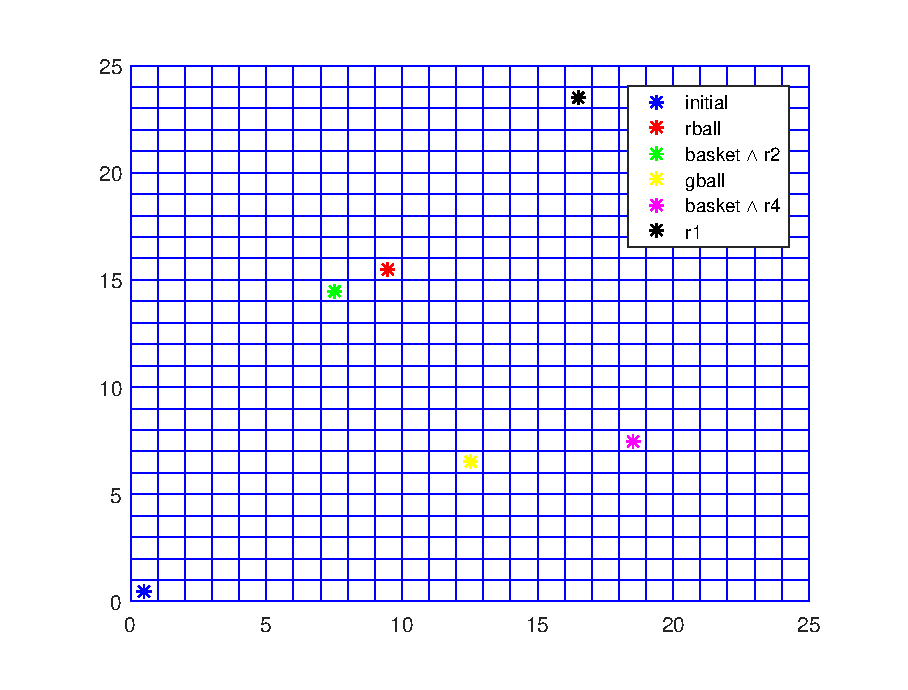
\includegraphics[scale=1]{workspace2.eps}
\label{fig:workspace2}
\caption{Workspace 2}
\end{figure}

We see that this is true in the output of the algorithms. Both give the same sequence of states and actions

%Have to recalculate this!!!!!!
The accepted algorithm gives \\


\begin{minipage}{\textwidth}
\begingroup
\fontsize{9pt}{12pt}\selectfont
\begin{lstlisting}
Accepted Algorithm
==================
accepted_plan done within 0.05s: precost 66.00, sufcost 0.00
\end{lstlisting}
\endgroup
\end{minipage} \\ \\


while the greedy algorithm gives \\


\begin{minipage}{\textwidth}
\begingroup
\fontsize{9pt}{12pt}\selectfont
\begin{lstlisting}
Greedy Algorithm
==================
greedy_plan done within 0.03s: precost 66.00, sufcost 0.00
\end{lstlisting}
\endgroup
\end{minipage} \\ \\


\section{Example 1 Overlapping Regions}
We now look at the same example, except now we have a different workspace. We choose this example to show what happens if the regions of interest are overlapping. Because of the way the code is structured, we are not able to make take transitions with two or more propositions at one time. We show the example if rball is in the same area as the basket. If this is the case, then pickrball and dropbasket could theoretically be done simultaneously. However, this is not possible because of the code. The only possible transitions that we can take that include \&\& have to be a region and a potential task. We leave the transitions satisfying this requirement and remove all others so the algorithm can have a better distances to follow. The automaton is now
\begin{figure}
\centering
\begin{tikzpicture}[->,>=stealth',shorten >=1pt,auto,node distance=3.5cm,
                    semithick]
  \tikzstyle{every state}=[fill=red,draw=black,text=black]

  \node[initial,state] (A)                    {$q_1$};
  \node[state] (B)                    [right of=A]{$q_2$};
  \node[state] (C)                    [right of=B]{$q_4$};
  \node[state] (E)                    [above of=B]{$q_3$};
  \node[state] (F)                    [above of=C]{$q_5$};
  \node[state,accepting]         (D) [right of=C] {$q_6$};

  \path (A) edge              node {pickrball} (B)
  		%(A) edge   [bend right=90]	 node {rball \&\& basket} (C)
  		%(E) edge		[near start]			node {rball \&\& basket} (C)
  		%(A) edge [loop above] node {$\neg \pi_1$} (A)
  		(B) edge [loop below] node {$\neg$ droprball} (B)
  		(B) edge              node {droprball} (C)
  		(A) edge              node {$\neg$pickrball} (E)
  		(E) edge              node {pickrball} (F)
  		(F) edge        [near end]      node {droprball} (C)
  		(C) edge [loop below] node {$\neg r1$} (C)
  		(C) edge              node {$r1$} (D)
  		(E) edge [loop above] node {$\neg$pickrball} (E)
  		(F) edge [loop above] node {$\neg$droprball} (F)
  		(D) edge [loop above] node {$r1$} (D);
\end{tikzpicture}
\caption{Simplified B\"uchi Automaton Corresponding to $\varphi = \diamond (\text{pickrball} \wedge \diamond \text{droprball}) \wedge \diamond \smallsquare r1$ 2}
\label{fig:ex1OverlapSimplifiedBuchi}
\end{figure} 

In this automaton, we now have $d(q_1)=3$, $d(q_2)=2$, $d(q_3)=3$, $d(q_4)=1$, $d(q_5) = 2$ and $d(q_6)=0$. We see again that rball and basket are not one step away from the initial node, implying that we cannot take the first step pickrball. This means that we can never go to $q_2$, and that there is only one path through the automaton to take. Therefore the greedy algorithm is guaranteed to compute the same path as the accepted algorithm and it will do so in less time.

We look at the results and see that the greedy algorithm indeed calculates the same path in a shorter amount of time than the accepted algorithm. \\


\begin{minipage}{\textwidth}
\begingroup
\fontsize{9pt}{12pt}\selectfont
\begin{lstlisting}
Accepted Algorithm
==================
accepted_plan done within 0.05s: precost 60.00, sufcost 0.00
...
full construction and synthesis done within 1.11s 
\end{lstlisting}
\endgroup
\end{minipage} \\ \\



\begin{minipage}{\textwidth}
\begingroup
\fontsize{9pt}{12pt}\selectfont
\begin{lstlisting}
==================
greedy_plan done within 0.02s: precost 60.00, sufcost 0.00

full construction and synthesis done within 1.09s 
\end{lstlisting}
\endgroup
\end{minipage} \\ \\


\section{Example 2}
We now look at the example taken from \cite{guo15} in which the robot has to pick up and deliver two different balls (rball and gball) to two different baskets, and the robot cannot carry two balls at once. After this is done the robot is to go to r1 and stay there. This task is formalized as 
\begin{align*}
\varphi = \diamond (\text{pickrball} \wedge \diamond (\text{droprball})) \wedge \diamond(\text{pickgball} \wedge \diamond (\text{dropgball})) \wedge \smallsquare (\text{pickrball} \rightarrow \\
 \textbf{X}(\neg \text{pickgball} \U \text{droprball})) \wedge \smallsquare (\text{pickgball} \rightarrow \textbf{X} (\neg \text{pickrball} \U \text{dropgball})) \&\& \diamond \smallsquare r1
\end{align*}
This formula formalizes the basket corresponding to rball is in region r2 and the basket corresponding to gball is in r4. The B\"uchi automaton corresponding to this formula is much to large to show. It has 75 states and 797 edges. If the reader is interested, the automaton can be found using the online tool \cite{ltlbuchiwebsite} with the input F(pickrball \&\& F(droprball)) \&\& F(pickgball \&\& F(dropgball)) \&\& G(pickrball -> X(! pickgball U droprball)) \&\& G(pickgball -> X(! pickrball U dropgball)) \&\& F(G(r1)). It is too large for the tool to give a visual representation but it will provide a list of states and edges.  

To analyse the performance of the greedy algorithm on this problem, we are going to break up this problem into the choices that the robot has. The robot has to pick up one of the balls, return it to the corresponding basket, then pick up the second ball and return it to its corresponding basket. Assuming that everything else is done in the optimal way, the only choice that must be made is which ball to pick up first. This is the output, accepted algorithm first: \\


\begin{minipage}{\textwidth}
\begingroup
\fontsize{9pt}{12pt}\selectfont
\begin{lstlisting}
Accepted Algorithm
==================
accepted_plan done within 0.63s: precost 118.00, sufcost 0.00
...
full construction and synthesis done within 55.25s 
\end{lstlisting}
\endgroup
\end{minipage} \\ \\


and the greedy algorithm \\


\begin{minipage}{\textwidth}
\begingroup
\fontsize{9pt}{12pt}\selectfont
\begin{lstlisting}
==================
greedy_plan done within 0.28s: precost 130.00, sufcost 0.00
...
full construction and synthesis done within 57.55s 
\end{lstlisting}
\endgroup
\end{minipage} \\ \\


as we can see, the greedy algorithm picks the closest ball (rball) first even though it is not optimal overall. The added cost is relatively small though, only 12. However, it is possible that the difference could be much larger. In an analysis of speed, the greedy algorithm does the search faster, In about half the time. In either case, the actual search takes around or less than a hundredth of the total time.

\section{Example 2 Modified}
We now look at a modified version of example two. Say the robot has to pick up and deliver two different balls (rball and gball) to two different baskets, and the robot cannot carry two balls at once and that is it. There is no need to go to r1, or do anything after the balls are returned to their respective baskets. This task is formalized as 
\begin{align*}
\varphi = &\diamond (\text{pickrball} \wedge \diamond (\text{droprball})) \wedge \diamond(\text{pickgball} \wedge \diamond (\text{dropgball})) \wedge \smallsquare (\text{pickrball} \rightarrow \\ 
& \textbf{X}(\neg \text{pickgball} \U \text{droprball})) \wedge \smallsquare (\text{pickgball} \rightarrow \textbf{X} (\neg \text{pickrball} \U \text{dropgball}))
\end{align*}
This version seems easier than original example. The B\"uchi automaton for this formula would seem to agree; it is smaller, with 38 nodes and 308 edges. However, here is the out put from both algorithms: \\


\begin{minipage}{\textwidth}
\begingroup
\fontsize{9pt}{12pt}\selectfont
\begin{lstlisting}
Accepted Algorithm
==================
accepted_plan done within 926.40s: precost 101.00, sufcost 0.00
...
full construction and synthesis done within 950.95s 
\end{lstlisting}
\endgroup
\end{minipage} \\ \\


and from the greedy algorithm \\


\begin{minipage}{\textwidth}
\begingroup
\fontsize{9pt}{12pt}\selectfont
\begin{lstlisting}
Greedy Algorithm
==================
greedy_plan done within 0.30s: precost 104.00, sufcost 0.00
...
full construction and synthesis done within 21.60s
\end{lstlisting} 
\endgroup
\end{minipage} \\ \\


This is by far the largest difference in computation times that we have seen thus far! We will show how this difference is caused by the searches from accepting nodes back to themselves.

As before, we have $|\text{product automaton}| =|\text{FTS}| \times |\text{B\"uchi}| \times |\text{possible actions}|$. The FTS still has 625 nodes, this buchi automaton has 38 nodes, and there are 5 possible actions ("none", "pickrball", "droprball", "pickgball", "dropgball"). This makes for a product automaton of 118750. There are 4 accepting states in the B\"uchi automaton. This gives us 12500 accepting nodes in the product automaton. The accepted algorithm calculates a path back from each accepting node back to itself. This calculation is relatively quick if the accepting node can transition back to itself; however, the cost is much longer if it doesn't. It turns out in this example only 629 of the accepting nodes have a self loop, while 11871 do not. It may seem like the accepting nodes should all be able to transfer back to themselves, but they cannot because of the accepting nodes in the B\"uchi automaton. 

Each accepting node in the B\"uchi automaton has a self loop however, the labels of the self loop can make many of these transitions impossible. The four self loop labels for the four accepting nodes of the B\"uchi automaton are (droprball \&\& dropgball), (!pickrball \&\& dropgball), (!pickrball \&\& !pickgball), and (droprball \&\& !pickgball). Thus the only possible self loop is (!pickrball \&\& !pickgball). All other accepting states must look for another path back to themselves, which results in the incredible increase in time. This is likely the largest danger and downside of using the accepted algorithm. The number of accepting states grows with the size of the FTS, the B\"uchi automaton, and the number of possible actions. Then we have to do a search for each of these accepting nodes.  



\section{Other Examples}
As we have seen, due to the complexity of the B\"uchi automata it can be very hard to analyse the performance of the greedy algorithm compared to the accepted algorithm with respect to cost for more complex formulas. We therefore provide the results of runs for various formulas in table \ref{table}. We use formulas from the table in \cite{somenzi00} to try to show a comprehensive experimentation. The formulas are run on the workspace in figure \ref{fig:workspace2}. 

\begin{landscape}
\begin{table}[]
\centering
\small
\begin{tabular}{|c|c|c|c|c|}
\hline
Formula & \makecell{Accepted Cost \\ prefix, suffix} & Accepted Time & \makecell{Our Cost \\ prefix, suffix} & Our Time \\ \hline
     '(!r223 U r445) || (!r268 U r435)'  &         27, 0     &      0.04         &      27, 0   &     0.01     \\ \hline
      '!r62 U(!r266 U r422)'  &         38, 0     &       0.05        &     38, 0     &     0.02     \\ \hline
       '[]<> r0 -> []<> r317' &         1, 0      &       5.06        &    1, 0      &    0.00     \\ \hline
       '[]<> r0 <-> []<> r317'  & 1, 0		&		10.70		& 1, 0 	&  0.00 \\ \hline 
      '!(<><> r498 <-> r541)' &	42, 0	&	0.03	&	42, 0	&	0.02	\\		\hline
      '!([]<> r3 -> []<>r591)' &	 3, 0	&	5.06 	&	3, 0 	&	0.00	\\		\hline
      '!([]<> r3 <-> []<>r591)' &	 3, 0	&	10.31	&	39, 0	&	0.01	\\		\hline
      '!r532 R (!r432 || r321)' &	 0, 0	&	4.97 	&	0, 0	&	0.01 	\\		\hline
     \makecell{ '<> r114 \&\& [](r114 -> <> r12) \&\& \\((X r114 U X r12) || !X( r114 U r12))' }&	24	&	0.08 	&	24	&	0.01	\\		\hline
   \makecell{ '<> pickrball \&\& [](pickrball -> <> droprball) \\ \&\& ((X pickrball U X droprball) || !X( pickrball U droprball))' } &	47, 0	&	28.87	&	47, 0	&	0.03	\\		\hline
      ' <> r124 \&\& <> !r124' &	28, 0	&	0.05 	&	28, 0	&	0.01	\\		\hline
%      &		&		&		&		\\		\hline
 %     &		&		&		&		\\		\hline
  %    &		&		&		&		\\		\hline
\end{tabular}
\caption{Comparison of Accepted Algorithm with Greedy Algorithm on Various Examples}
\label{table}
\end{table}
\end{landscape}

As we can see, our algorithm always produces a path in a shorter time than the accepted algorithm. However, it can happen that our algorithm produces a plan that is much worse than the accepted algorithm e.g.\ '!([]<> r3 <-> []<>r591)'. 

%\subsection{OR Operator}
%As we have seen in the LTL semantics, LTL formulas can contain an OR Boolean connective i.e.\ $\varphi = \varphi_1 \lor \varphi_2$. In all the other examples that we have seen, the formulas specify tasks and the algorithm has to \textit{at most} choose the order of the tasks. The OR connective introduces the idea that the algorithm has to choose \textit{which} tasks to do. Let us first look at the formula $(\diamond \pi_0 \wedge \diamond \pi_1 ) \lor \diamond \pi_2$.
%The B\"uchi automaton corresponding to this formula as calculated by \cite{gastin01} is shown in figure \ref{fig:ORbuchi}.
%
%\begin{figure}
%\centering
%\begin{tikzpicture}[->,>=stealth',shorten >=1pt,auto,node distance=4cm,
%                    semithick]
%  \tikzstyle{every state}=[fill=red,draw=black,text=black]
%
%  \node[initial,state] (A)                    {$q_1$};
%  \node[state] (B)                    [right of=A]{$q_2$};
%  \node[state] (C)                    [right of=B]{$q_4$};
%  \node[state] (E)                    [below of=C]{$q_3$};
%  \node[state] (F)                    [above of=C]{$q_5$};
%  \node[state,accepting]         (D) [right of=C] {$q_6$};
%
%  \path (A) edge              node {$\neg (\pi_0 \lor \pi_1 \lor  \pi_2)$} (B)
%  		(B) edge   				 node {$\pi_0$} (C)
%  		(B) edge					node {$\pi_1$} (E)
%  		(A) edge					 node {$\neg \pi_2$} (F)
%  		(C) edge 					node {$\pi_1$} (D)
%  		(B) edge              node {$\pi_0$} (C)
%  		(E) edge              node {$\pi_0$} (D)
%  		(F) edge              node {$\pi_2$} (D)
%  		(A) edge              [bend left] node [near end] {$\pi_0$} (C)
%  		(A) edge             node {$\pi_1$} (E)
%  		(A) edge              [bend left] node {$\pi_2$} (D);
%  		%(E) edge [loop above] node {$\neg$rball} (E)
%  		%(F) edge [loop above] node {$\neg$basket} (F)
%  		%(D) edge [loop above] node {$r1$} (D);
%\end{tikzpicture}
%\caption{Simplified B\"uchi Automaton Corresponding to $(\diamond \pi_0 \wedge \diamond \pi_1 ) \lor \diamond \pi_2$}
%\label{fig:ORbuchi}
%\end{figure} 
%
%The distances corresponding to this automaton are $d(q_1) = 1$, $d(q_2) = 2$, $d(q_3)=1$, $d(d_4)=1$, $d(q_5)=1$ and $d(q_6)=0$. As one can see, starting with a distance of 1, the only lower level is 0, which is the accepting level. Therefore our algorithm will only do one Dijkstra search, which is the same as the accepted algorithm. Our algorithm therefore gives the optimal result. 

%\begin{figure}
%\centering
%\begin{tikzpicture}[->,>=stealth',shorten >=1pt,auto,node distance=3.5cm,
%                    semithick]
%  \tikzstyle{every state}=[fill=red,draw=black,text=black]
%
%  \node[initial,state] (A)                    {$q_1$};
%  \node[state] (B)                    [right of=A]{$q_2$};
%  \node[state] (C)                    [below of=B]{$q_3$};
%  \node[state] (D)                    [right of=B]{$q_4$};
%  \node[state] (E)                    [above of=D]{$q_5$};
%  \node[state] (F)                    [right of=C]{$q_6$};
%  \node[state] (G)                    [below of=F]{$q_7$};
%  \node[state,accepting]         (H) [right of=D] {$q_8$};
%
%  \path (A) edge              node {$\neg (\pi_0 \lor \pi_1 \lor  \pi_2 \lor \pi_3)$} (B)
%  		(A) edge   				 node {$\neg (\pi_0 \lor \pi_1 \lor  \pi_2 \lor \pi_3)$} (C)
%  		(A) edge					node {$\pi_0$} (E)
%  		(A) edge			[bend left] node {$\pi_1$} (D)
%  		(A) edge 					node {$\pi_2$} (F)
%  		(A) edge             [bend right] node {$\pi_3$} (G);
%%  		(E) edge              node {$\pi_0$} (D)
%%  		(F) edge              node {$\pi_2$} (D)
%%  		(A) edge              [bend left] node {$\pi_0$} (C)
%%  		(A) edge             node {$\pi_1$} (E)
%%  		(A) edge              [bend left] node {$\pi_2$} (D);
%  		%(E) edge [loop above] node {$\neg$rball} (E)
%  		%(F) edge [loop above] node {$\neg$basket} (F)
%  		%(D) edge [loop above] node {$r1$} (D);
%\end{tikzpicture}
%\caption{Simplified B\"uchi Automaton Corresponding to $(\diamond \pi_0 \wedge \diamond \pi_1 ) \lor (\diamond \pi_2 \wedge \diamond \pi_3)$}
%\label{fig:ORbuchi}
%\end{figure} 
